\documentclass[12pt]{elsart}
\usepackage{amsmath}
\usepackage{amssymb}
\usepackage{program}
\usepackage{graphicx}
\newcommand{\field}[1]{\mathbb{#1}}

\usepackage{algorithm}
\usepackage{algpseudocode}

%%%%%%%%%%%%%%%%%%%%%%%%%%%%%%%%%%%%%%%%%Space to make more readable!
%\vspace{10 mm}
%%%%%%%%%%%%%%%%%%%%%%%%%%%%%%%%%%%%%%%%%Take out later!

\begin{document}

\pagestyle{empty}

\begin{center}
\Large  CS5463 Fundamentals of Software  \\
\large {\bf Homework 3}\\
\normalsize Due 10/30/20 before 11:59pm (Central Time)
\end{center}


{\bf 1.  Arrays and Heaps (6 points)}

\begin{enumerate}
\item (3 points) Suppose you wanted to create an algorithm to find the number of elements $\geq k$ in an array, $A$, of $n$ distinct elements.  

Specifically, describe efficient algorithms to solve this problem when $A$ is the following data structures.  

\begin{enumerate}
   \item Unsorted array
   \item Sorted array   
   \item Max-heap
\end{enumerate}

  \item (3 points) Analyze the runtime of your three algorithms from the previous part:

\begin{enumerate}
   \item Unsorted array
   \item Sorted array   
   \item Max-heap
\end{enumerate}

\end{enumerate}

{\bf 2. Huffman Encoding  (2 points)}

\begin{enumerate}
 \item Show the process by which a Huffman tree would be built for the following string of character: (i.e., redraw the tree after each new node is created).

\begin{quote}
 ``cannercancanacanra"
\end{quote}

 \item Using your tree, find the encoding that would result for the above string.
\end{enumerate}

{\bf 3.  Red-Black Trees (2 points)}

\begin{enumerate}
\item Company X has created a new variant on red-black trees which also uses blue as a color for the nodes.  They call these ``red-black-blue trees".  Below are the new rules for these trees:\\

\begin{itemize}
   \item Every node is red, blue, or black.
   \item  The root is black.
   \item Every leaf (NIL) is black.
   \item If a node is red, then both its children are black.
   \item If a node is blue, then both its children are red or black.
   \item For each node, all simple paths from the node to descendant leaves contain the
same number of black nodes.\\
\end{itemize}

\begin{enumerate}
   \item (2 points) In class we found that the height, $h$, of a red-black tree is $\leq 2\log_2(n+1)$ (where $n$ is the number of keys).  Find and prove that a similar bound on height of the red-black-blue trees.
\\\\({\bf Hint:} You can use the same approach as we did to show\\ $h \leq 2\log_2(n+1)$).\\

   \item (0 points - just for fun) Adding an additional color didn't seem to improve our bound on $h$ (i.e., 3 colors allows the tree to become more unbalanced than with 2 colors).    What benefit might we get from the extra color?
\end{enumerate}

\end{enumerate}

{\bf 4.  B-trees (4 points)}

\begin{enumerate}
   \item (2 points) Show the results of inserting the keys\\\\
$E,F,G,U,V,W,H$\\\\
in order into the B-tree shown below.  Assume this B-tree has minimum degree $k=2$. Draw only the configurations
of the tree just before some node(s) must split, and also draw the final configuration.

\vspace{-1.5mm}
\begin{figure}[h]
	\centering 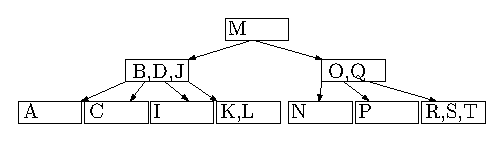
\includegraphics[width=0.7\textwidth]{BTreeProblem-01}
\end{figure}
\vspace{-1.5mm}

   \item (2 points) Suppose you have a B-tree of height $h$ and minimum degree $k$. What is the largest number of keys that can be stored in such a B-tree?  Prove that your answer is correct.
\\\\({\bf Hint:} Your answer should depend on $k$ and $h$. This is similar to \\theorem we proved in the B-tree notes).
\end{enumerate}


{\bf 5.  Hash Table Probabilities (3 points)}

\begin{enumerate}
   \item (1 point) Suppose $2$ keys are inserted into an empty hash table with $m$ slots. Assuming
simple uniform hashing, what is the probability of:
\begin{enumerate}
   \item exactly $0$ collisions occurring
   \item exactly $1$ collisions occurring\\
\end{enumerate}

   \item (2 points) Suppose $3$ keys are inserted into an empty hash table with $m$ slots. Assuming
simple uniform hashing, what is the probability of:
\begin{enumerate}
   \item exactly $0$ collisions occurring
   \item exactly $1$ collisions occurring
   \item exactly $2$ collisions occurring
\end{enumerate}

\end{enumerate}


{\bf 6.  Hash Table (7 points)}

\begin{enumerate}
   \item Consider inserting the keys $2, 21, 3, 58, 11, 42, 34$ into a hash
table of length $m = 10$ with the hash function $h(k) = k \bmod 10$.
\begin{enumerate}
   \item (2 points)  Illustrate the result of inserting these keys using linear probing to resolve collisions.
   \item (2 points) Illustrate the result of inserting these keys using chaining to resolve collisions.
\end{enumerate}

   \item Consider inserting the keys $8,5,14$ into a hash
table of length $m = 8$ with the hash function $h(k) = \lfloor m(kA - \lfloor kA\rfloor)\rfloor$ where $A=0.625$.
\begin{enumerate}
   \item (2 points) Illustrate the result of inserting these keys.
   \item (1 point) Now compute the hash function of the key $14$ using the alternative algorithm described below.  
\\\\You can assume we have a word size $w=4$. Since $m=8=2^3$, $p=3$.  Since $A=0.625=10/2^4=10/2^w$, $s=10$.
\\\\{\bf Alternative Algorithm:} Compute $ks$ and convert it to a binary number.  This number will consist of $\leq 2w$ bits.  Look at the rightmost $w$ bits.  Of those bits, convert the leftmost $p$ bits back to an integer.  This integer is your hash table slot.\\
\end{enumerate}



\end{enumerate}

\end{document}